\documentclass[crop,tikz]{standalone}

\usetikzlibrary{
	chains,
	positioning,
	arrows.meta,
	decorations.pathreplacing,
	calc,
	fit,
	shapes.geometric
}

\begin{document}

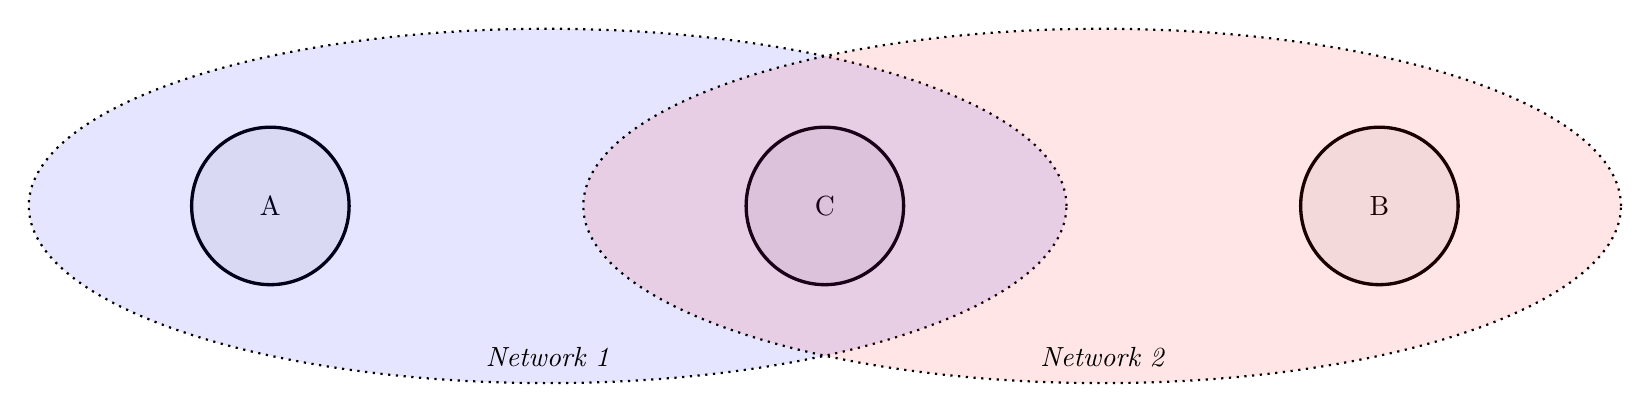
\begin{tikzpicture}[
	nwknode/.style={
		circle,
		very thick,
		minimum size=2cm,
		draw,
		fill=black!5,
	},
	network/.style args = {#1/#2}{
		ellipse,
		minimum height=4.5cm,
		draw,
		thick,
		dotted,
		fill=#1,
		fill opacity=0.1,
		text opacity=1,
		label={[anchor=south,above=1mm]270:{\itshape Network #2}}
	},
]
	\node[nwknode] (A) {A};
	\node[nwknode] (C) [right=5cm of A] {C};
	\node[nwknode] (B) [right=5cm of C] {B};
	
	\node[network={blue/1}, fit=(A)(C)] (net1) {};
	\node[network={red/2},  fit=(C)(B)] (net2) {};

\end{tikzpicture}

\end{document}